\chapter{Introduction to Bioinformatics}
\label{chap:intro}

This chapter offers an overview of the bioinformatics field, focusing on key molecular biology concepts. It covers proteins, their sequences and structures, ligands, binding sites (including cryptic binding sites), major biological databases and file formats, and widely used tools for visualization, binding site prediction, and structural analysis.

\section{Proteins, Ligands, Amino Acids}
\label{sec:proteins}

\textbf{Proteins} are vital macromolecules involved in numerous biological functions, such as catalyzing biochemical reactions, offering structural support, and regulating cellular activities.

They consist of \textbf{amino acids} connected by \textbf{peptide bonds}, forming \textbf{polypeptide chains}. Amino acids are molecules containing an amino group (\(-NH_2\)), a carboxyl group (\(-COOH\)), and a unique side chain (\(R\) group) that determines the amino acid's properties. The sequence of these amino acids in a polypeptide chain is known as the \textbf{primary structure} of a protein. The sequence of the protein determines its function \cite{nelson2008lehninger}, \cite{voet2010biochemistry}. There are \textbf{20 standard amino acids}, each possessing distinct characteristics that affect protein folding and interactions. In this thesis, we will focus on the 20 standard amino acids, which are the building blocks of proteins, although many more non-standard amino acids are used in drug discovery and development \cite{dumas2015designing}.

\begin{figure}[ht]
    \centering
    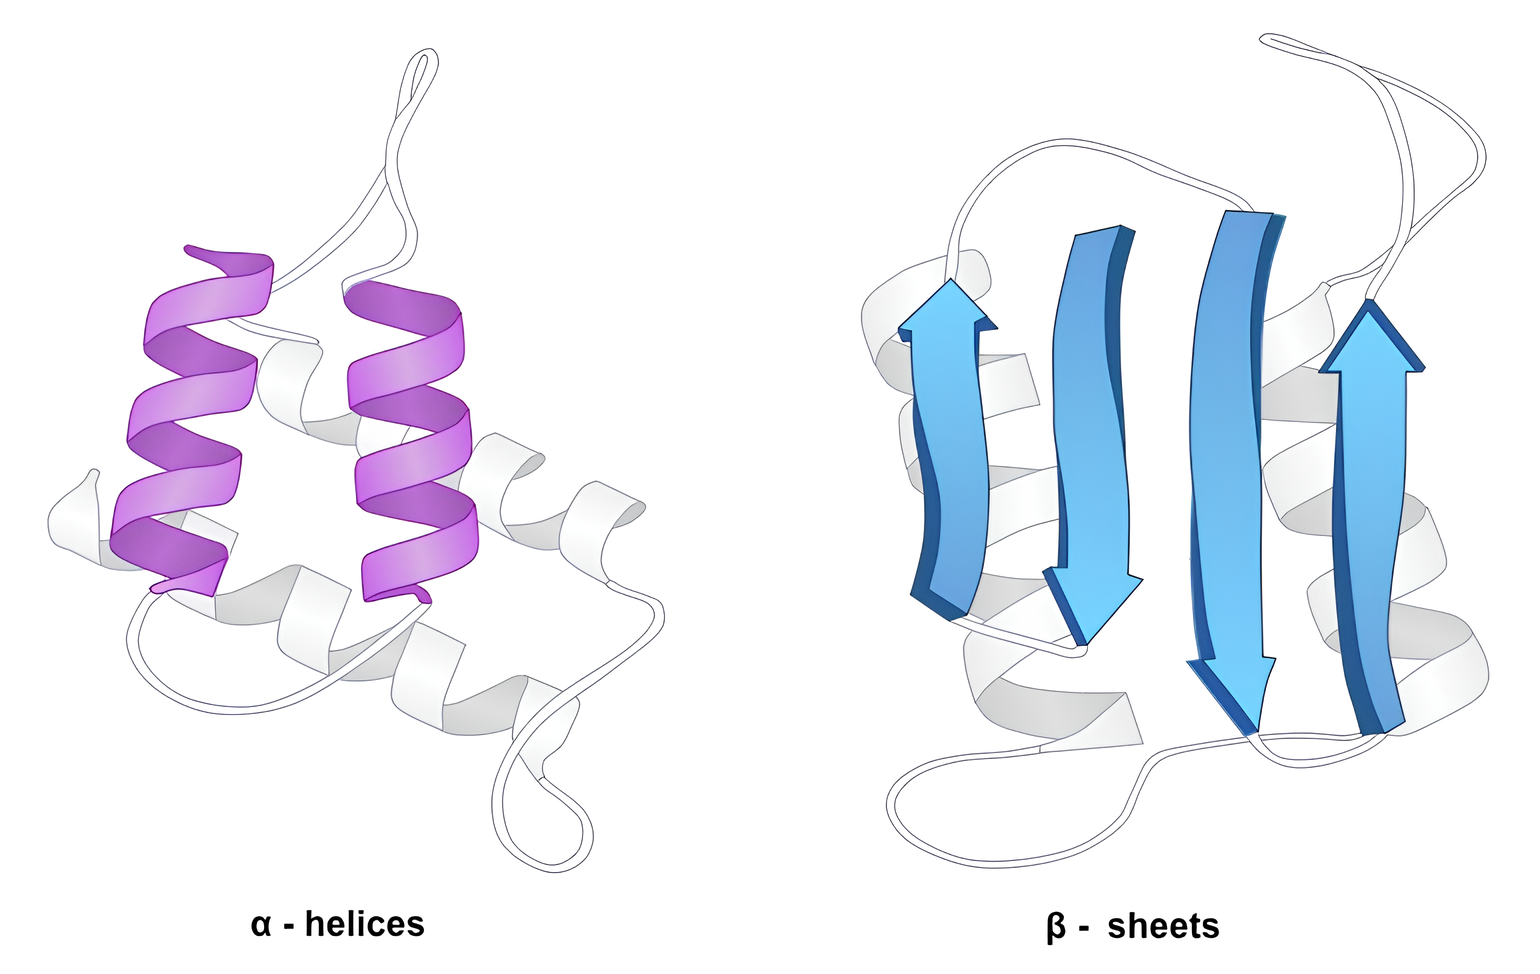
\includegraphics[width=0.8\textwidth]{img/ah_bs.png}
    \caption{Illustration of an alpha helix and a beta sheet, the two most common types of protein secondary structure. Generated with DALL·E 3.}
    \label{fig:alpha-beta}
\end{figure}

The second level of protein structure is the \textbf{secondary structure}, which refers to local folding patterns within the polypeptide chain. The most common secondary structures are \textbf{alpha helices} and \textbf{beta sheets}, as shown in Figure~\ref{fig:alpha-beta}. These structures arise from hydrogen bonding between the backbone atoms of the amino acids, stabilizing the overall protein structure. All proteins also have a \textbf{three-dimensional (3D) structure}, also known as \textbf{tertiary structure}, which is crucial for their function \cite{nelson2008lehninger}, \cite{voet2010biochemistry}.

The tertiary structure is determined by the interactions between the side chains of the amino acids, including hydrophobic interactions, hydrogen bonds, ionic bonds, and disulfide bridges. The final level of protein structure is the \textbf{quaternary structure}, which refers to the assembly of multiple polypeptide chains into a functional protein complex \cite{nelson2008lehninger}, \cite{voet2010biochemistry}.

In the past, the tertiary and quaternary structures of proteins were determined through experimental methods such as X-ray crystallography and nuclear magnetic resonance (NMR) spectroscopy \cite{berman2000protein}. However, with the advent of deep learning and artificial intelligence, it is now possible to predict protein structures from their amino acid sequences. The most notable example is AlphaFold \cite{jumper2021highly}, \cite{abramson2024accurate}, a deep learning model developed by DeepMind that has achieved remarkable accuracy in predicting protein structures and has been widely adopted in the field of bioinformatics. AlphaFold provides a per-residue confidence metric called the predicted Local Distance Difference Test (plDDT) score\footnotemark[1], which indicates the reliability of the predicted atomic positions. In recognition of the profound impact of these advances, the Nobel Prize in Chemistry was awarded in 2024 for the development of methods for the prediction of protein structures using artificial intelligence \cite{abriata2024nobel}. Other notable tools introduced in the past months include Boltz-2 \cite{passaro2025boltz2} and Chai-1 \cite{chai2024chai}. Today, predicted structures often closely match experimental results, as illustrated in Figure~\ref{fig:alphafold-vs-exp}.

\footnotetext[1]{The predicted Local Distance Difference Test (plDDT) score is a per-residue confidence metric output by AlphaFold, indicating the reliability of the predicted atomic positions; higher values suggest greater confidence. In the color scheme, blue indicates the most confident regions, while orange/yellow depict less confident regions.}

\begin{figure}[ht]
    \centering
    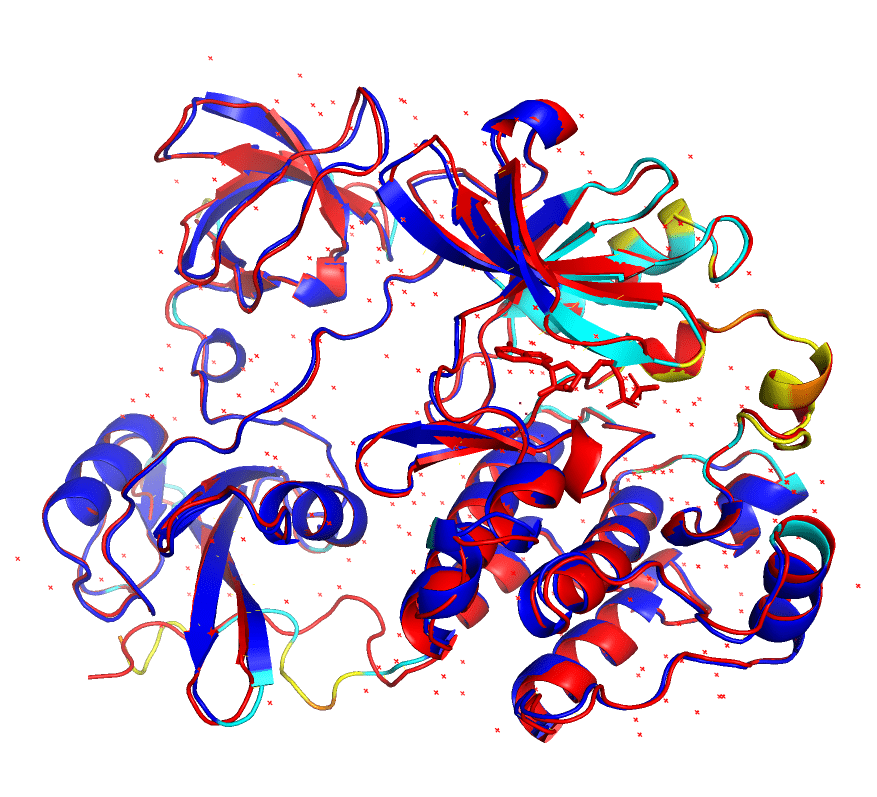
\includegraphics[width=0.8\textwidth]{img/alphafold_vs_exp.png}
    \caption{Comparison of AlphaFold predicted structure and experimental structure of the protein 2SRC (Crystal Structure of Human Tyrosine-Protein Kinase C-SRC, in Complex with AMP-PNP). The predicted structure is shown in blue to yellow colors (depicting the plDDT score), while the experimental structure is shown in red. The two structures are nearly identical after the alignment, demonstrating the accuracy of AlphaFold predictions. Image from PyMOL.}
    \label{fig:alphafold-vs-exp}
\end{figure}
\par

Protein function is largely determined by interactions with other molecules, known as ligands. These may be small molecules, ions, or other proteins that bind to specific regions, often resulting in conformational or functional changes. Such interactions are crucial for processes like enzymatic catalysis, signal transduction, and immune responses. In drug discovery, identifying and characterizing these sites is important, with computational approaches aiding both new therapeutic development and drug repurposing. Additionally, de novo protein design allows for the creation of proteins with tailored functions, often guided by predictive tools such as AlphaFold before experimental testing \cite{huang2016coming}.

\section{Binding Sites, Cryptic Binding Sites (CBSs)}
\label{sec:binding-sites}

\textbf{Binding sites} are defined regions on a protein where ligands interact and bind. These sites typically correspond to cavities or grooves on the protein surface and are frequently linked to conformational changes that influence protein function. Proteins with a ligand bound are termed \textbf{holo} proteins, while those without a ligand are known as \textbf{apo} proteins. In holo proteins, the binding site is identified by the position of the ligand, but even apo proteins may contain several potential binding sites.

\textbf{Cryptic binding sites (CBSs)} are regions on proteins that are not visible or accessible in the unbound (apo) structure but can form and become available for ligand binding following conformational changes. These sites typically appear only after ligand interaction or other molecular events induce structural rearrangements. Computational methods such as CryptoBench \cite{vskrhak2025cryptobench} have been created to predict cryptic binding sites. A significant contribution in this area is CryptoSite \cite{cimermancic2016cryptosite}, which leverages known apo-holo protein pairs to identify CBSs, offering an alternative to time-consuming molecular dynamics simulations.

\section{Databases, File Formats}
\label{sec:dbs-formats}

This section provides an overview of the key bioinformatics databases for protein structures and introduces the main file formats used in this field.

\subsection{RCSB PDB}
\label{sec:rcsb-pdb}

The RCSB PDB (Research Collaboratory for Structural Bioinformatics Protein Data Bank) \cite{berman2000protein}, often referred to simply as the "PDB database", is the primary repository for experimentally determined protein, nucleic acid, and macromolecular complex structures. It serves as a foundational resource for bioinformatics, with many machine learning and deep learning models relying on its data for training and validation. The database is publicly accessible at \url{https://www.rcsb.org/} and offers a REST API for programmatic data access. As of June 2025, the PDB contains over 238,000 structures. Many organizations also maintain local, enriched copies of the PDB. The open sharing of structural data is encouraged, as it supports the development and improvement of computational models used throughout the scientific community \cite{callaway2025alphafold}.

\subsection{AlphaFold Database}
\label{sec:alphafold-db}

The AlphaFold Database \cite{varadi2024alphafold} contains over 200 million protein structures predicted by the AlphaFold model. While the majority of these structures have not been experimentally validated, those with high pLDDT scores are considered reliable. It is important to note that certain protein regions, known as intrinsically disordered regions, may exhibit low pLDDT scores due to their inherent flexibility and lack of stable structure. The database is publicly available at \url{https://alphafold.ebi.ac.uk/}.

\subsection{UniProt Database}
\label{sec:uniprot-db}

The UniProt database \cite{uniprot2025uniprot} is a comprehensive resource for protein sequences and functional information. It provides detailed annotations for proteins. The records, also called UniProt accessions, are often used with PDB and AlphaFold entries to provide further context about the protein's strcuture. UniProt is available at \url{https://www.uniprot.org/}. A part of the UniProt database is the UniProt Knowledgebase (UniProtKB), which contains two sections: UniProtKB/Swiss-Prot, which includes manually curated entries with high-quality annotations, and UniProtKB/TrEMBL, which contains automatically annotated entries that have not yet been reviewed \cite{boutet2016uniprotkb}.

\subsection{PDB File Format}
\label{sec:pdb-format}

The PDB (Protein Data Bank) file format is a text-based format used to represent three-dimensional structures of biological molecules, primarily proteins and nucleic acids. It contains information about atom coordinates, connectivity, b-factors, and other structural details. Each PDB file should start with header lines providing metadata about the structure, such as the structure name, authors, methods used and additional comments. Then, the atomic coordinates are listed in a list of ATOM and HETATM records, which specify the atom type, residue name, chain identifier, residue sequence number, and the x, y, z coordinates of each atom in the structure. The PDB format might include information about secondary structure elements, such as helices and sheets \cite{westbrook2003pdb}. Some of the information might be ommited, especially in the case of working with structures generated by deep learning methods, such as RFDiffusion \cite{watson2023novo}.

\begin{figure}[H]
    \centering
    \lstinputlisting[caption={
        An edited example of a PDB file containing information about a protein structure generated by RFDiffusion.
    }]{code/rfdiff_example.pdb}
\end{figure}


\subsection{mmCIF File Format}
\label{sec:mmcif-format}

The mmCIF (Macromolecular Crystallographic Information File) format is a more modern and flexible alternative to the PDB format, designed to overcome the limitations of the PDB format, especially for large structures \cite{bourne199730}. The PDB database, mentioned in Section~\ref{sec:rcsb-pdb}, has been transitioning to the mmCIF format for new entries. Although it is encouraged to use mmCIF for new structures, many existing tools and databases still rely on the PDB format thanks to its simpler format.

\subsection{FASTA File Format}
\label{sec:fasta-format}

The FASTA file format is a widely used, text-based format for representing biological sequences, such as proteins or nucleic acids. Each sequence entry begins with a header line that starts with a ">" character, followed by a description or identifier. The sequence itself is written on the following lines, typically using single-letter codes. Multiple sequences can be included in a single FASTA file, each with its own header. While the header line is commonly present, it is technically optional, which allows easy creation of FASTA files \cite{lipman1985rapid}.

\begin{figure}[H]
    \centering
    \lstinputlisting[
        caption={
            An example of a FASTA file containing information about the 6A5J sequence (containing only 13 amino acids).
        },
        breaklines=true
    ]{code/fasta_example.fasta}
\end{figure}

\section{Related Tools, Projects}
\label{sec:related-tools}

\subsection{PrankWeb}
\label{sec:prankweb}

\subsection{AHoJ}
\label{sec:ahoj}

\subsection{PyMOL}
\label{sec:pymol}

\subsection{Mol*}
\label{sec:molstar}

\subsection{CryptoBench}
\label{sec:cryptobench}

\subsection{CryptoSite}
\label{sec:cryptosite}

